\documentclass[]{elsarticle} %review

\usepackage{lineno}
\usepackage{hyperref}
\usepackage{amsmath}
\usepackage[english]{babel}
\usepackage{graphicx}
\usepackage{fullpage}

\usepackage{xcolor}
\modulolinenumbers[5]

\journal{Journal of \LaTeX\ Templates}

%%%%%%%%%%%%%%%%%%%%%%%
%% Elsevier bibliography styles
%%%%%%%%%%%%%%%%%%%%%%%
%% To change the style, put a % in front of the second line of the current style and
%% remove the % from the second line of the style you would like to use.
%%%%%%%%%%%%%%%%%%%%%%%

%% Numbered
%\bibliographystyle{model1-num-names}

%% Numbered without titles
%\bibliographystyle{model1a-num-names}

%% Harvard
%\bibliographystyle{model2-names.bst}\biboptions{authoryear}

%% Vancouver numbered
%\usepackage{numcompress}\bibliographystyle{model3-num-names}

%% Vancouver name/year
%\usepackage{numcompress}\bibliographystyle{model4-names}\biboptions{authoryear}

%% APA style
%\bibliographystyle{model5-names}\biboptions{authoryear}

%% AMA style
%\usepackage{numcompress}\bibliographystyle{model6-num-names}

%% `Elsevier LaTeX' style
\bibliographystyle{elsarticle-num}
%%%%%%%%%%%%%%%%%%%%%%%

\newcommand{\Kn}{\mathrm{Kn}}
\newcommand{\dd}{\mathrm{d}}
\newcommand{\pder}[2][]{\frac{\partial#1}{\partial#2}}
\newcommand{\pderdual}[2][]{\frac{\partial^2#1}{\partial#2^2}}
\newcommand{\pderder}[3][]{\frac{\partial^2#1}{\partial#2\partial#3}}
\newcommand{\Pder}[2][]{\partial#1/\partial#2}
\newcommand{\Pderdual}[2][]{\partial^2#1/\partial#2^2}
\newcommand{\Pderder}[3][]{\partial^2#1/\partial#2\partial#3}
\newcommand{\Set}[2]{\{\,{#1}:{#2}\,\}}
\newcommand{\OO}[1]{O(#1)}
\newcommand{\transpose}[1]{#1^\mathsf{T}}
\newcommand{\dxi}{\boldsymbol{\dd\xi}}
\newcommand{\bxi}{{\boldsymbol{\xi}}}
\newcommand{\dx}{\boldsymbol{\dd{x}}}
\newcommand{\bx}{\boldsymbol{x}}

% topic-specific
\newcommand{\equil}[1]{#1^\mathrm{(eq)}}
\newcommand{\refer}[1]{#1_0}
\newcommand{\todo}[1]{\textcolor{olive}{#1}}

\graphicspath{{pics/}}

\begin{document}

\begin{frontmatter}

\title{Fluid--kinetic coupling based on lattice-Boltzmann and discrete-velocity methods under the finite-volume formulation}

%% Group authors per affiliation:
\author{V.V.Aristov}
%%\address{}

%% or include affiliations in footnotes:
\author{O.V. Ilyin}
%%\ead[url]{www.elsevier.com}

\author{O.A. Rogozin}
%%\cortext[mycorrespondingauthor]{Corresponding author}
%%\ead{support@elsevier.com}

%%\address[mymainaddress]{1600 John F Kennedy Boulevard, Philadelphia}
%%\address{360 Park Avenue South, New York}

\begin{abstract}

In the present paper, a novel hybrid fluid--kinetic computational approach based on the discrete-velocity (DV)
approximation including lattice-Boltzmann (LB) technique is proposed.
\todo{Numerical schemes for a kinetic equation are used in regions of rarefied flows and LB schemes are used in continuum flow zones.}
Different characteristics and possibilities of these schemes are considered.
\todo{The important issues devoted to matching solutions in buffer cells are discussed.}
\todo{(Grad's Gauss--Hermite quadrature). The expansion of the solution on Hermite polynomials is used.}
The Couette-flow problem are investigated as a test problem.
The good correspondence with the benchmark solution is obtained.
Influence of different parameters on the accuracy of the hybrid solutions is analyzed.
A special attention is paid to the recent high-order LB models.
\todo{The hybrid scheme with these lattices permit to study dissipative values, in particular, heat flux.}
\todo{Different variants of LBM are considered and the efficiency of the hybrid method is evaluated. We show that the results of the hybrid method are with very close to the well-known tabulated solutions of the Couette flow.
The methodological investigation is made concerning different aspects constructing a hybrid scheme for 1D Couette flow. The criteria transformation from the continuum region to kinetic one is proposed. The influence of the point transformation is studied. The CPU time for the hybrid scheme and for BGK scheme is evaluated. Different lattice schemes are used.}

\end{abstract}

\begin{keyword}
discrete-velocity method, lattice-Boltzmann method, rarefied and continuum flows, BGK equation, hybrid scheme
\end{keyword}

\end{frontmatter}

\linenumbers

\section{Introduction}\label{sec:intro}

Introduction

So far a problem of effective numerical simulation of complex flows is challenging despite the efforts of many researchers). This is due, in particular, to a multiscale complicated structure of a flow where there are zones of equilibrium and nonequilibrium states. The use of the kinetic equation in all regions is very computationally consuming. On the other hand, the modern approaches including the LB method is a profitable tool for description near-equilibrium flows, but it is not adequate for regions where the distribution function is not close to Maxwellian. So the computational hydrodynamics is being confronted with an issue of constructing the unified numerical method suited for calculations in all regions of flows.

(rewrite. without classification. not only three).
One of the most effective methods for modeling multiscale flows is the construction of hybrid schemes. Until now all the developed hybrid methods can be divided into three types. The methods of the first type include the solution of both kinetic and hydrodynamic equations in the entire spatial region, and the transport coefficients for the hydrodynamic equations are calculated on the basis of the distribution function. In the methods of the second type, the separation of the velocity space in the subdomains of slow and fast molecules is used, and these regions are processed separately from each other (see e.g. \cite{Kolobov2013}). The third type includes methods with dividing the physical space region into kinetic and continual subregions using some criterion of domain decomposition.\cite{Dimarco2014}.

In methods of the third type, approaches of DSMC type in the kinetic zones and the Euler or Navier-Stokes equations in the continuum are used, but the usual statistical modeling in the buffer zone yields appreciable statistical noise (especially for subsonic flows), which complicates calculations. Unlike DSMC, the methods of direct numerical solution of the Boltzmann equation do not give a statistical noise of macroscopic parameters. Therefore, hybrid methods based on a direct numerical solution of the Boltzmann equation appear in principal to be more promising. \cite{Staso2016short, Staso2016long, Staso2018}.

A novel hybrid kinetic approach (of the third type) for multiscale problems is proposed in the present paper. The kinetic-based description of continuum media has been suggested independently and has been widely used since the beginning of 80s, see~\cite{Potkin1975, Pullin1980, Reitz1981, Aristov1983}. Later these kinetic-consistent schemes have been developed in~\cite{Elizarova1985, Deshpande1986, Prendergast1993, Chou1997, Ohwada2002, Ohwada2004Xu, Ohwada2004Kobayashi, Ohwada2006}. Such methods reproduce the Euler and Navier–Stokes (NS) dynamics. The cellular-automata approximation for the Navier–Stokes equations has been developed in the middle of 80s (see e.g.~\cite{Frisch1986}). Finally, the lattice-gas model based on the BGK equation was proposed in the beginning of 90s (see e.g.~\cite{Qian1992}). It gave rise to a wide class of mentioned numerical methods called LB methods (see e.g.~\cite{Succi2001}).

The fluid-kinetic coupling is an effective approach for the description of multiscale flows. The coupling of the Boltzmann and Euler (or NS) equations is one of canonical example of such hybrid schemes (see, e.g., \cite{Bourgat1996} \cite{Tallec1997}) and has been also elaborated and applied within the framework of UFS (Unified Flow Solver) \cite{Kolobov2007}.

The other hybrid schemes have been developed in recent years, see e.g. \cite{Xu2010} Some works are based on alternative proposals (in particular for DSMC) related to the properties of the distribution functions. In \cite{Larina2005} the authors proposed a method in which the distribution function is represented by the sum of a local Maxwellian and a nonequilibrium term that has the order of magnitude of the low Knudsen number.


\todo{LB method is based, in fact, on some DV models of DV method. Therefore, it is natural to connect DV and LB methods. In the present paper, we attempt to couple DV method for the Boltzmann equation (or its BGK model) and LB method for the Navier--Stokes equations. The first one adequately describes nonequilibrium regions, while the second one provides an adequate description in continuum-flow regions.} There are obvious relations between these two methods. For instance, one can cite a phrase from \cite{Rivet2001}: ''This type of discrete kinetic theory can be seen as the ''ancestor'' of the lattice gas approach''. The LB method is genetically related to the Broadwell-type models~{\cite{Broadwell1964shock, Gatignol1975}, which use small numbers of discrete velocities to caricature the Boltzmann dynamics. Thus the DV approximation is a natural basis for construction a hybrid fluid--kinetic model.

The DV schemes with the large number of discrete velocities are used in direct methods for solving BE, BGK, S-model or other kinetic equations. The DV method is applied with the combination of Monte Carlo or quasi-Monte Carlo procedures for evaluating collision integrals and for computing the appropriate moments which are used in the collision integrals of the model kinetic equations. For the near-equilibrium zones the small number of discrete velocities can be considered. Therefore, one can expect that LB approaches are fit for describing flows in these regions.

At the boundaries of the BGK and LBGK domains the coupling method is applied. For mapping we assume that in the overlapping zone of the two methods the distribution function takes the form of truncated Grad expansion. In the mapping domain the Lattice Boltzmann distribution function is equivalent to the Grad expansion via Gauss-Hermite quadrature. This approach of mapping has been suggested in~\cite{Staso2016short, Staso2016long} where the solution is obtained by means of hybridization of the DSMC and LB methods (see also a new work~\cite{Staso2018}).

The plan of the present paper is as follows.
The employed kinetic equations and nondimensional variables are introduced in Section~\ref{sec:equations}.
The numerical methods are described in Section~\ref{sec:numerics}.
This section is subdivided in several parts in which in particular the coupling procedure of the hybrid algorithm is presented.
In Section~\ref{sec:results} examines the computations obtained by the BGK model in the whole region of the Couette flow, the analogous results by the different LB models and by the hybrid scheme. The efficiency of the hybrid approach is presented.
In section~\ref{sec:summary} Conclusions and a perspective development of DV hybrid methods is discussed.


\section{Basic equations}\label{sec:equations}

%%% Nondimensional variables
Let \(L\), \(\refer\rho\), \(\refer{T}\), \(V = \sqrt{2R\refer{T}}\) and \(\refer{p} = \refer{\rho}R\refer{T}\) be
the reference length, density, temperature, velocity, and pressure, respectively.
The specific gas constant \(R = k_B/m\), where \(k_B\) is the Boltzmann constant and \(m\) is the molar mass.
Then, \(f\refer{\rho}/V^D\) is the one-particle velocity distribution function (VDF)
defined in \((2D+1)\)-dimensional space \((tL/V, x_iL, \xi_iV)\) and
the macroscopic variables take the following form:
\(\rho\refer{\rho}\) is the density, \(v_iV\) is the velocity, \(T\refer{T}\) is the temperature,
\(p_{ij}\refer{p}\) is the stress tensor, \(q_i\refer{p}V\) is the heat-flow vector.
In the dimensionless form, they are calculated as polynomial moments of VDF:
\begin{equation}\label{eq:macro}
    \begin{gathered}
    \rho = \int f \dxi, \quad
    v_i = \frac1{\rho} \int \xi_i f \dxi, \quad
    T = \frac{2}{D\rho}\int(\xi_i-v_i)^2 f \dxi = \frac{p_{ii}}{D\rho}, \\
    p_{ij} = 2 \int(\xi_i-v_i)(\xi_j-v_j) f \dxi, \quad
    q_i = \int(\xi_i-v_i)(\xi_j-v_j)^2 f \dxi.
    \end{gathered}
\end{equation}

%%% Boltzmann equation
The VDF is governed by the Boltzmann equation
\begin{equation}\label{eq:Boltzmann}
    \pder[f]{t} + \xi_i\pder[f]{x_i} = \frac1kJ(f),
\end{equation}
where \(J(f)\) is the collisional operator and \(k=\refer\mu V/\refer{p}L\)
is expressed in terms of the reference gas viscosity \(\refer\mu\).
The Knudsen number \(\Kn=\lambda/L = 2k/\sqrt\pi\), where \(\lambda\) is the mean free path.
\begin{equation}\label{eq:equilibrium}
    \equil{f} = \frac{\rho}{(\pi T)^{D/2}}\exp\left(-\frac{(\xi_i - v_i)^2}T\right)
\end{equation}
is a local Maxwellian as the equilibrium function.
%\begin{equation}\label{eq:Knudsen_number}
%    \Kn = \frac2{\sqrt\pi} k
%    k = \frac{\sqrt\pi}2\Kn = \frac{\refer\mu V}{\refer{p}L}.
%\end{equation}

%%% Model equation
In the present paper, we restrict ourselves to the simplest relaxation model~\cite{Krook1954, Welander1954}
\begin{equation}\label{eq:bgk}
    J(f) = \frac1\tau\left(\equil{f}-f\right), \quad \tau = \frac{T^{\omega-1}}{\rho},
\end{equation}
often referred as the Bhatnagar--Gross--Krook (BGK) model of the Boltzmann equation.
\(\omega\) is the exponent of the viscosity law of the gas.
The nonlinearity in \(\equil{f}\) is more severe in comparison to the full Boltzmann equation
since \(\equil{f}\) depends on \(f\) via its moments,
but the BGK model is much simpler from the numerical point of view.

\section{Numerical method}\label{sec:numerics}

The equation \eqref{bgk} is solved by the second-order splitting scheme into the transport equation \textcolor{red}{(DO NOT UNDERSTAND  THE PHRASE)}
$$
\frac{\partial f}{\partial t}+\mathbf{v}\frac{\partial f}{\partial \mathbf{x}}=0,
$$
for which a finite-volume method with an explicit second-order TVD scheme is used, and the space-homogeneous BGK equation
$$
\frac{\partial f}{\partial t}=\frac{{1}}{\tau Kn}(\Phi-f)
$$
which has the exact solution
$$
f=\Phi+e^{t/\tau Kn}(f_0-\Phi).
$$
\textcolor{red}{(THEN WHAT ?)}
The three-dimensional velocity space is discretized by the uniform lattice confined with the sphere of radius \(\zeta_{\max}=4\).
\(M=16\) nodes are placed along each axis. The total amount of nodes is equal to \(6528\).

The  second  approach is  called the  Lattice Boltzmann method which is the further simplification of the BGK model \cite{Succi2001}. We assume that the considered flow is  slow,  i.e the  Mach number is  close  to zero and isothermal, then we  can expand  the local Maxwell term $\Phi$
in the Taylor series on the bulk velocity $\mathbf{u}$  up to the terms of the second order. Moreover, we assume that  the particle can travel with the  velocities $\mathbf{c}_i$ from a finite discrete set of possible velocities.
Finally the general LBGK model is  obtained  by the finite difference integration of the BGK equations on the  characteristics jointly with the aforementioned assumptions
$$
f(t+\delta t, \mathbf{x}+\mathbf{c}_j\delta t, \mathbf{c}_j)-f(t, \mathbf{x},\mathbf{c}_j)=
$$
\begin{equation}\label{lbgk}
=\frac{1}{(\frac{1}{2}+\frac{\tau Kn}{\delta t})}\left\{ \rho w_j\left(1+ \frac{\mathbf{c_j}\mathbf{u}}{c_s^2}+\frac{(\mathbf{c_j}\mathbf{u})^2-c_s^2u^2}{2c_s^4}\right)-f(t,\mathbf{x}, \mathbf{c}_j) \right \},
\end{equation}
for $j=1\ldots N$, where $\mathbf{c}_j$ are lattice velocities, $c_s$  is  sound velocity defined by $\sum_jw_j\mathbf{c}^2_j=c_s^2$, $w_j$ are  lattice weights (or discrete analogs of the Maxwell state) obeying $\sum_jw_j=1$, $\tau$  is  relaxation time, $\delta t$  is lattice  time step and  $N$  is number of lattice velocities. The  lattice weights and  velocities should be evaluated in a such way that at the $Kn \rightarrow 0$ limit the resulting Navier-Stokes equations  are reproduced with negligible  errors if the flow is slow ( of order $Ma^3$). The integration on  the  characteristics using the trapezium rule adds the small error terms of the  order  $\delta t^2$.


Several approaches can be applied for the  construction of the LB models like Gauss-Hermite \cite{He1997},\cite{Shan1998}, \cite{Shan2006},\cite{Shan2010} and the entropic  method \cite{Karlin1999},\cite{Chikatamarla2006},\cite{Chikatamarla2009}.

We adopt the spatial domain splitting procedure  for solving  the  boundary problems  for  rarefied gas dynamics.
Commonly the  non-equilibrium effects in flows appear near boundaries, therefore the  boundary domains are modeled with the BGK model while the internal  zone which is modeled with the Lattice BGK. Previously, the  approach based on solving  the gas  dynamics with DSMC method and LBGK models using  domain splitting was presented in papers \cite{Staso2016short, Staso2016long} where  the Couette and  Poiseuille  flow  was  considered. Nevertheless, LBGK and DSMC coupling leads to appearance  of some  noise \cite{Staso2016short} therefore the  introduction of the LBGK and  BGK coupling  method  is  very desirable.



We will discuss the   matching  procedure   in the spatial overlapping  zone  of the BGK and LBGK methods.
First of all, we  assume that in this  domain  the real distribution function of the gas is close  to the Maxwell state with zero bulk velocity,  unit temperature and  can  be casted in the  form of the truncated  Grad expansion
\begin{equation}\label{grad}
f_{Grad}(\mathbf{y},\mathbf{v})=\frac{1}{\sqrt{(2\pi})^3}\exp\left(-\frac{\mathbf{v}^2}{2}\right)\left(a(\mathbf{x})
+\sum_{j}a_j(\mathbf{x})H_{j}+\frac{1}{2}\sum_{jk}a_{jk}(\mathbf{x})H_{jk}\right),
\end{equation}
 where $H_j, H_{jk}$ are the  Hermite polynomials of the first and second order defined by
  $$
H_j(\mathbf{v})=\frac{(-1)}{w(\mathbf{v})}\frac{\partial}{\partial v_j}w(\mathbf{v}),  \quad H_{jk}(\mathbf{v})=\frac{1}{w(\mathbf{v})}\frac{\partial^2}{\partial v_j\partial v_k}w(\mathbf{v})
$$
and
 $$
 w(\mathbf{v})\equiv \frac{1}{\sqrt{(2\pi})^3}\exp\left(-\frac{\mathbf{v}^2}{2}\right).
 $$
 The  terms $a, a_j,a_{jk}$ are coefficients depending on $\mathbf{y}$ (the point in the overlapping domain). We suppose  that the truncation of the  Grad expansion at the  second order terms is  minimal  but sufficient  possibility since  the Navier-Stokes  equations  can be reproduced  for this  case with small errors of order $Ma^3$  when Knudsen number  tends  to zero.
 We will use the function \eqref{grad} for the transfer of the boundary data between the lattice Boltzmann  and the BGK models. We will discuss this  procedure  in turn.

For the sake of clarity we  assume  that the flow  depends  not on the whole vector $\mathbf{y}$ but on one of the coordinates only, we denote  it  by $y$.

At the  first  step we  update the BGK distribution function $f_{BGK}(y_{\mathbf{\alpha}},\mathbf{v}_{\mathbf{\beta}})$ (where we define $y_{\mathbf{\alpha}},\mathbf{v}_{\mathbf{\beta}}$ as the BGK difference scheme's spatial points and velocities) for the velocities with positive (non-positive) $v_y$ component  in the whole BGK domain using the boundary data on the wall (see Fig. 3 in the case  of the Couette flow, the computations of the BGK scheme starts  at $y=0.5$). In the spatial domain where  the BGK method overlaps the LBGK method we map the BGK  scheme distribution on the Grad distribution function by calculating the following coefficients $a, a_j,a_{jk}$ using  the formulas below
\begin{equation}\label{bgk_to_grad}
a(y_{\mathbf{\beta}})=\sum_{\mathbf{\beta}}  f_{BGK}(y_{\mathbf{\alpha}},\mathbf{v}_{\mathbf{\beta}}),   \quad a_j(y_{\mathbf{\beta}})=\sum_{\mathbf{\beta}}f_{BGK}(y_{\mathbf{\alpha}},\mathbf{v}_{\mathbf{\beta}})H_j(\mathbf{v}_{\mathbf{\beta}}), \quad  a_{jk}(y_{\mathbf{\beta}})=\sum_{\mathbf{\beta}}f_{BGK}(y_{\mathbf{\alpha}},\mathbf{v}_{\mathbf{\beta}})H_{jk}(\mathbf{v}_{\mathbf{\beta}}).
\end{equation}
Once  this summation is performed we are able to recover  the Grad  distribution function \eqref{grad} in the considered spatial domain.

Next we will map the distribution \eqref{grad} on the lattice Boltzmann distribution using  the  Gauss-Hermite quadrature method.
The idea of the method is based on the fact  that the representation of the distribution function in the  Grad form  is equivalent to the  lattice  Boltzmann method \cite{He1997},\cite{Shan1998}, \cite{Shan2006}.
We  consider the first moments $a,a_j,a_{jk}$  in the integral form and then calculate them using Gauss-Hermite quadratures
$$
\{a,a_j,a_{jk}\}=\int f_{Grad}(\mathbf{v})\{1,H_j(\mathbf{v}),H_{jk}(\mathbf{v})\}d\mathbf{v}=\sum_{s}w_s\frac{f_{Grad}(\mathbf{v}_s)}{w(\mathbf{v}_s)}
\{1,H_j(\mathbf{v_s}),H_{jk}(\mathbf{v_s})\},
$$
where $w_s, \mathbf{v}_s$  are the weights  and the  nodes of the Gauss-Hermite quadrature respectively. The  nodes $\mathbf{v}_s$  can be  considered as  the  lattice Boltzmann velocities while $ w_s\frac{f(\mathbf{v}_s)}{w(\mathbf{v}_s)}$ are the lattice Boltzmann distribution function values and
$w_s$ are the  lattice analog of the total Maxwell distribution.  Then the  formula
\begin{equation}\label{grad_to_latt}
f_{latt,s}\equiv w_s\frac{f_{Grad}(\mathbf{v}_s)}{w(\mathbf{v}_s)}
\end{equation}
gives  the mapping from  the Grad truncated distribution function $f_{Grad}$ to the lattice Boltzmann distribution function $f_{latt,s}$ for the correspondent speeds $\mathbf{v}_s$. Now having  the  boundary values we  update the lattice Boltzmann distribution function $f_{latt,s}$  for the  velocities $\mathbf{v}_s$  with positive  $y$  component (non-positive).
%\begin{figure}[!h]
%\centering
%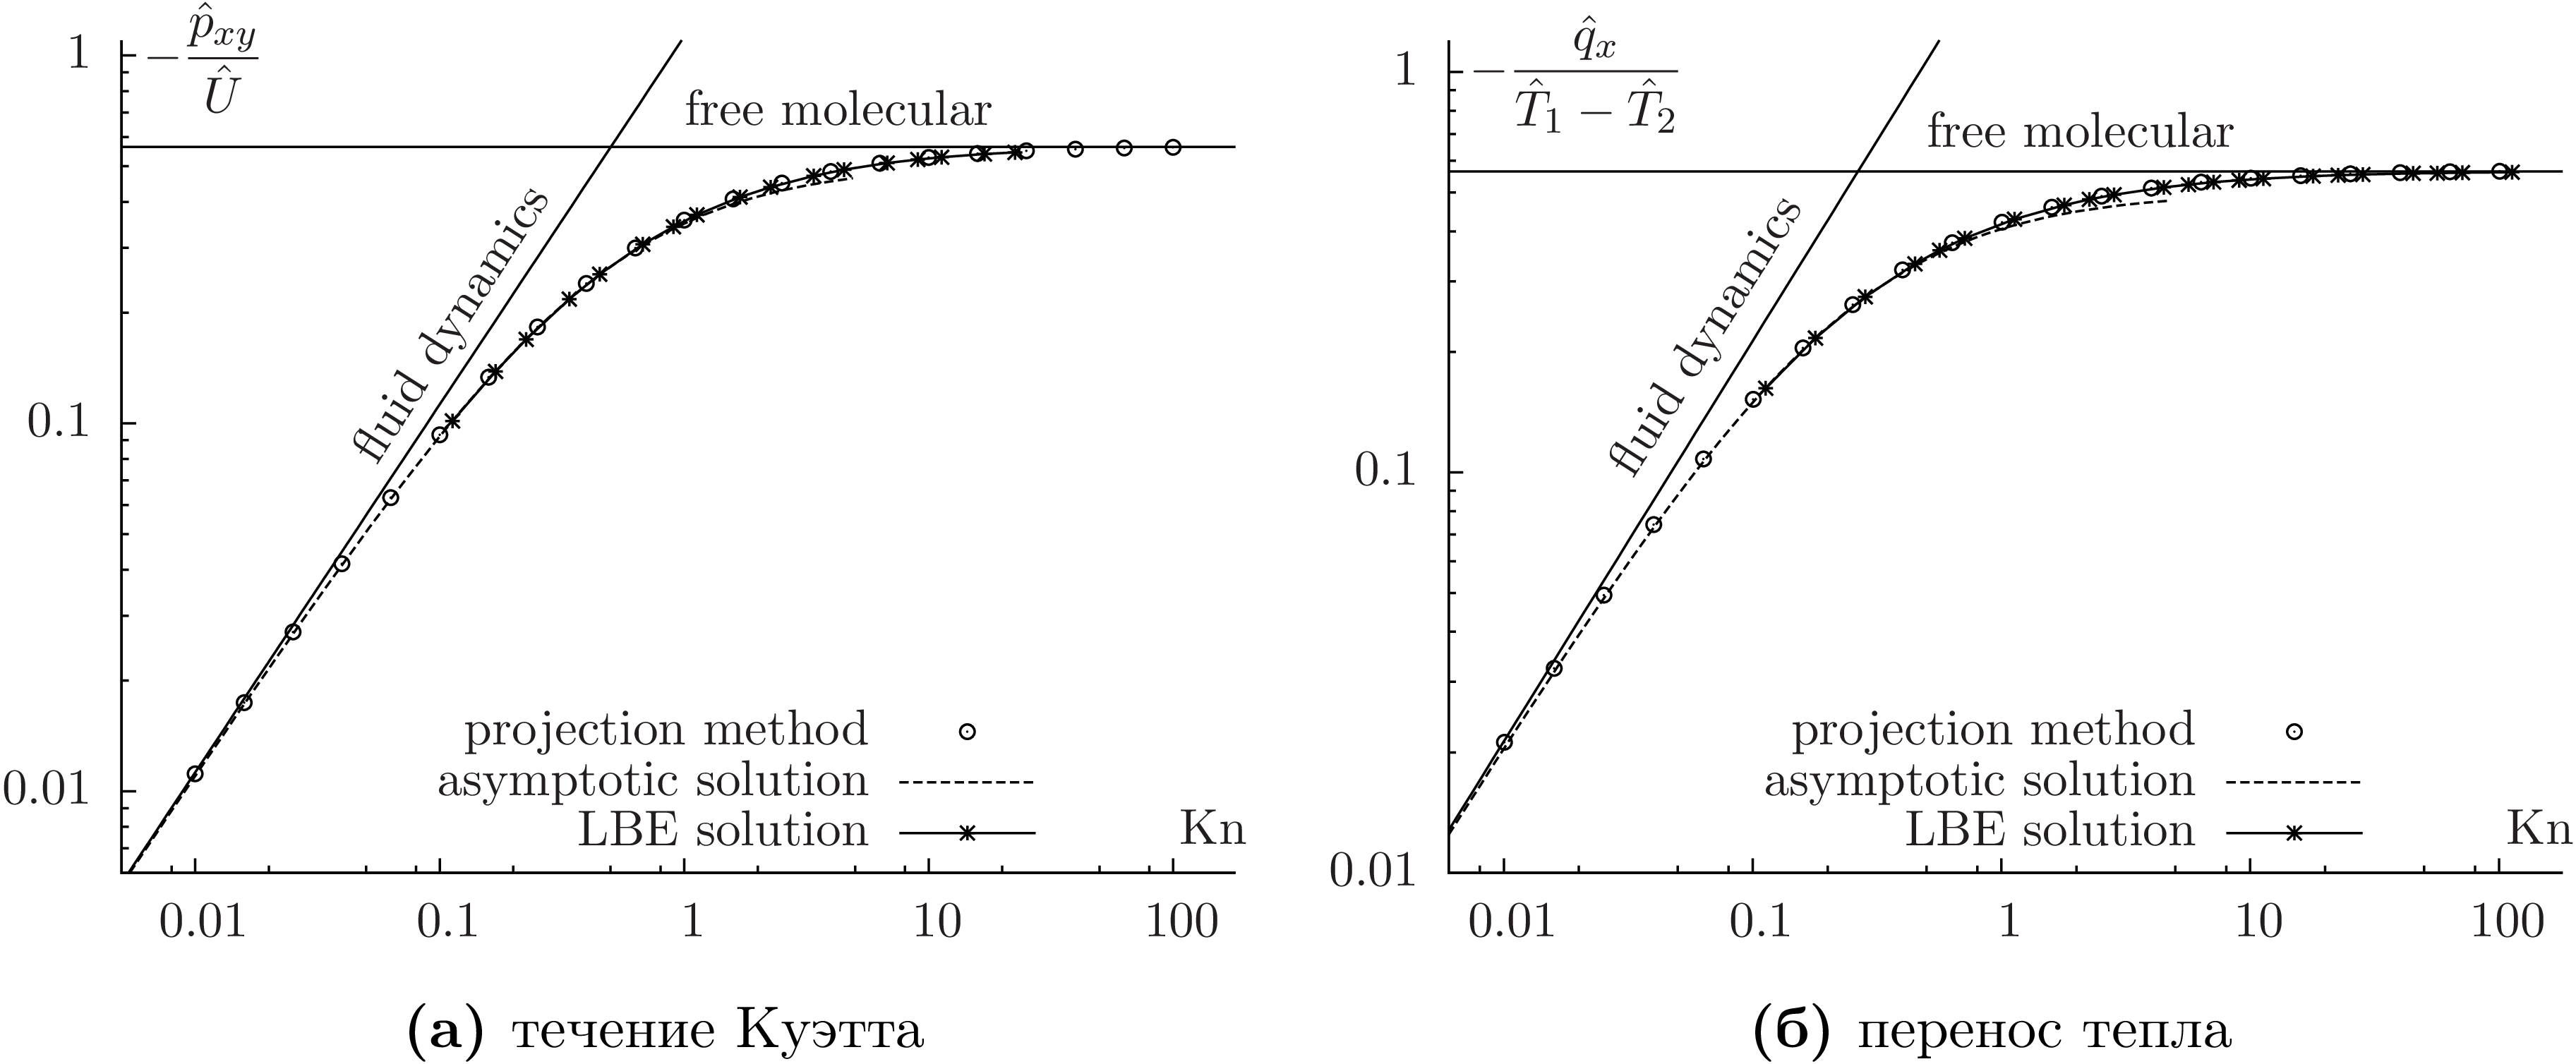
\includegraphics[height=60mm]{fig1.jpg}
%\caption{Step 1 of the  mapping  scheme.}
%\end{figure}
%\begin{figure}[!h]
%\centering
%\includegraphics[height=60mm]{fig2.jpg}
%\caption{Step 2 of the  mapping  scheme.}
%\end{figure}

The  second  step consists of the evaluation of the  distribution functions for the non-positive  (positive) velocities. Now we  start
from the  another boundary and using  the  boundary  conditions  we calculate the Lattice  Boltzmann distribution for the velocities with non-positive  $y$-component (positive) in LBGK spatial domain. Next we evaluate the moments $a,a_j,a_{jk}$ and finally  recover  the  Grad  distribution function. We have
$$
a=\sum_sf_{latt,s}, \quad a_j=\sum_sf_{latt,s}H_j(\mathbf{v}_s), \quad  \quad a_{jk}=\sum_sf_{latt,s}H_{jk}(\mathbf{v}_s).
$$
Now  we  are ready derive the BGK distribution function in the  BGK and  LBGK  overlapping domain. This  can be made by a simple
discretization of the Grad distribution functions at  the  nodes  of the  BGK difference scheme. Finally, we evaluate the BGK distribution function for  the  all velocities  with non-positive  $y$-component (positive) in BGK spatial domain.


\begin{figure}[!h]
\centering
\includegraphics[height=80mm]{dvm.pdf}
\caption{The  results of the  numerical study for the BGK nonlinear model $\Delta v=0.02, Kn=0.1$. The  black boxes correspond  to the  tabulated theoretical solutions \cite{Luo2015, Luo2016}. The  point $y=0.5$ corresponds  to the position of the right plane, the point $y=0$ lies in the middle between the moving planes.}
\end{figure}

%\begin{figure}[!h]
%\centering
%\includegraphics[height=80mm]{lbm.pdf}
%\caption{\textcolor{red}{ABSCISSAE IS X HERE !?!}The  results of the  numerical study for the Lattice Boltzmann D3Q19 model $\Delta v=0.02, Kn=0.1$. The  black boxes correspond  to the  tabulated theoretical solutions \cite{Luo2016}. The departure of the  LBGK bulk velocity form the  theoretical values is  observed in the Knudsen layer. The  point $y=0.5$ corresponds  to the position of the right plane, the point $y=0$ lies in the middle between the moving planes.}
%\end{figure}

\begin{figure}[!h]
\centering
\includegraphics[height=80mm]{d3q19.pdf}
\caption{The  results of the  numerical study for the Lattice Boltzmann D3Q19 model $\Delta v=0.02, Kn=0.1$. The  black boxes correspond  to the  tabulated theoretical solutions \cite{Luo2015, Luo2016}.  The  matching  point is  located at $y=0.38$. The  point $y=0.5$ corresponds  to the position of the right plane, the point $y=0$ lies in the middle between the moving planes.}
\end{figure}

\begin{figure}[!h]
\centering
\includegraphics[height=80mm]{hyb-d3q19-narrow.pdf}
\caption{The  results of the simulation for the matching point at $y=0.44$ for D3Q19+BGK model.}
\end{figure}

\begin{figure}[!h]
\centering
\includegraphics[height=80mm]{hyb-d3q19-wide.pdf}
\caption{The  results of the simulation for the matching point at $y=0.26$ for D3Q19+BGK model.}
\end{figure}


\begin{figure}[!h]
\centering
\includegraphics[height=80mm]{d3v64.pdf}
\caption{The  results of the simulation for the matching point at $y=0.38$ for D3Q64.}
\end{figure}


\begin{figure}[!h]
\centering
\includegraphics[height=80mm]{d3v96.pdf}
\caption{The  results of the simulation for the matching point at $y=0.38$ for D3Q96.}
\end{figure}


\begin{figure}[!h]
\centering
\includegraphics[height=80mm]{d3q121.pdf}
\caption{\textcolor{red}{CAN ONE EXPLAIN THE STRANGE RESULT ?} The  results of the simulation  for D3Q121.}
\end{figure}



\begin{figure}[!h]
\centering
\includegraphics[height=80mm]{hyb-d3v96.pdf}
\caption{\textcolor{red}{WHY HYBRID IS EVEN WORSE THAN THE SOLE  MODEL}The  results of the simulation for the matching point at $y=0.38$ for D3Q96+BGK model.}
\end{figure}



\section{Results of numerical simulations}\label{sec:results}

\todo{In the present paper, we deal with the flow between the two parallel planes which have non-zero relative velocity (the plane Couette flow) for small Knudsen numbers. For solving this problem we develop a hybrid BGK and LBGK coupling method. The gas dynamics in Knudsen layers is considered using the full nonlinear BGK equation while the internal zone is described by LB model.}

The classical stationary Couette problem has been used as a test for the consideration of the hybrid BGK+LBM BGK scheme. The results of the computations for BGK in the whole 1D computational domain are compared with the computations with the LBM and BGK scheme and with the computations by the hybrid scheme. The gas is confined between two infinite parallel plates placed at $y = \pm 1/2$ with constant temperature $T = 1$ and velocities ($v = \pm\Delta v/2,0,0$). A complete diffuse reflection are assumed at the plates. The average density is equal to unity $\int_{-1/2}^{1/2}\rho dy=1$. The physical space $0 < y < 1/2$ is divided into $N = 40$ nonuniform cells refined near $y = 1/2$. This numerical example was tested for the Knudsen number Kn=0.1. The results of the TVD difference scheme for thee BGK  are presented in Fig.1. The buffer layer is located for \textcolor{red}{the first variant} of computation at a distance of $1.2$ mean free path from the plate. The point of matching has been defined as the boundary between the Knudsen layer and the continuum zone of the flow, of course the switching procedure should be introduced, e.g. by the magnitudes of some moment gradients, in our calculations changing the coupling point has been investigated.

\textcolor{red}{(THE DETAILS OF THE  OVERLAPPING  BETWEEN THE DOMAINS SHOULD BE REVEALED)  }

The results of the simulations for the Lattice BGK  (D3Q19) in the whole spatial domain are showed in Fig. 2. One can see the differences for the velocity profile between the LBGK and the tabulated data. Obviously the lattice Boltzmann  model is  unable to describe  the  boundary layer with a good precision.
The  heat flux for lattice Boltzmann model equals zero in the whole domain since this model can not tackle with the third  moment.   We use  the  kinetic (diffusive) boundary conditions at the wall, for the LB models  this boundary condistions are described in
\cite{ansumali2002}. More  precisely, let us define $U_w, c_w^2$  as the wall velocity and  the wall temperature and $\mathbf{n}$ is  the wall inward normal vector, then we  have
\begin{equation}\label{kinet_bound}
f_{latt, s}=
\frac{\sum_{\mathbf{v}_j\mathbf{n}<0} f_{latt,j}|\mathbf{v}_j\mathbf{n}|}{\sum_{\mathbf{v}_j\mathbf{n}<0}
f^{eq}_j|\mathbf{v}_j\mathbf{n}|}f^{eq}_s, \quad  \mathbf{v}_s \mathbf{n}>0,
\end{equation}
where
$$
f^{eq}_{j}=\rho w_j\left(1+ \frac{\mathbf{v_j}\mathbf{U}_w}{c_w^2}+\frac{(\mathbf{v_j}\mathbf{U}_w)^2-c_w^2U_w^2}{2c_w^4}\right).
$$
 The formula  \eqref{kinet_bound}  allows to evaluate  the reflected distribution $\mathbf{v}_s\mathbf{n}>0$ if the  impinging distribution $\mathbf{v}_s\mathbf{n}<0$ is  known.

 The computations by the hybrid method LBGK(D3Q19)+BGK show good correspondence with the tabulated data except of the heat flux which equals zero in the lattice Boltzmann domain, see Fig. 3.

We have the preliminary results regarding the hybrid scheme’s efficiency. The typical CPU time for the BGK(DVM) $\sim 16$ s, the typical CPU time for LBM (D3Q19) $\sim 4$ s, zone of BGK (DVM) $\sim 1/4$ of the total zone, zone of LBM (D3Q19) $\sim 3/4 $ of the total zone, CPU time for BGK in the hybrid scheme $\sim 4$ s, CPU time for LBM (D3Q19) in the hybrid $\sim 3$ s, CPU time of the hybrid $\sim 7$ s, so the efficiency of the hybrid is more than $2$ times.

\begin{figure}[!h]
\centering
\includegraphics[height=80mm]{acceleration.pdf}
\caption{The hybrid method acceleration. $N_0$ is the number of spatial points in the Knudsen layer.\textcolor{red}{HAVE  NO IDEA  WHY THE INCREASE IN NUMBER  OF CELLS AFFECTS THE PRODUCTION}}
\end{figure}

\textcolor{blue} {Hybrid simulations with different positions of the matching points have been also considered and presented in Figs. 4-5.}
\textcolor{blue} {Results of more accurate computations for obtaining the efficiency are presented in Fig. 4.It is important that this efficiency tends to the limit when increasing the number of nodes in the coordinate computational domain. It is obvious because the number of velocity nodes is negligible in comparison with that in BGK and the limit is determined by the ratio of the number of coordinate points in the entire computational domain to the number of coordinate points in the kinetic region with computations on the basis of BGK}

More complex LBM (see ??)  are also considered and results in Figs.  are compared with the standard  well-known LBM schemes with small velocity points.

The last considered simulations for hybrids with more complex LBM are very important because allow us to describe dissipative values namely the heat flux. In Fig. ?? the mentioned macroscopic parameters are showed for the Lattice Model D3Q96. One can see that the heat flux is reproduced by the LBM in the middle continuum zone.

\textcolor{blue} {The criteria of the distinguishing between continuum and rarefied zones according to the value of the heat flux can be used. The threshold value for the transition from the continuum region to the kinetic region could be, e.g. related to the accepted level of the error in the calculations. Namely, if the module of the heat flux is less than this threshold value than this region is related to the continuum area and vice versa. In Fig. 5 the value related to the mentioned criteria is shown for all points of the coordinate computational domain.}

\section{Conclusions}\label{sec:summary}

In the paper, we presented a new algorithm  of merging of the numerical solutions for BGK kinetic equation  applied in the boundary regions with the Lattice Boltzmann Models used in continuum regions. The buffer cells use the distribution function in a form of the Grad expansion, that allows us to construct a hybrid method. We applied several lattice Boltzmann models ranging from the most common D3Q19 to LBM models with the large numbers (in comparison with ordinary samples) of  velocities [1] capable to simulate some dissipative properties. This method was tested for a simple one-dimensional Couette problem for the isothermal  regime.   The following problems for the further study can be addressed.
 The usage of multiple velocities in the  difference  schemes  for the full Boltzmann equation or BGK equation is somewhat overkill since  the highest moments  can be unimportant for many flows then the methods for the velocity number reduction for the methods should be developed.  Moreover the implementation of the  Cartesian grids and the advection part in a fashion similar  to LB method potentially allows to diminish the interpolation errors in the finite difference expressions for the Boltzmann equation. In [2] a similar idea has been realized for D3Q27 in the advection part of BE.
The other developments could be concerned to the hybrid method for supersonic flows, see , e.g. a recent paper [3] Implementation of the entropic lattice models has been applied in the hybridization scheme like D3Q41-ZOT Ansumali, Chikatamarla, Karlin- many papers]. Potentially the usage of entropic models is very appealing due to its amazing stability for low viscosities (and large Reynolds numbers). In recent papers [3, 5-6] the LBM method extended to thermal, compressible and supersonic  flows with appropriate lattices  and  this models  can be also considred as  candidates in hybrid methods.


%%% old


Perspectives of hybrid DVM schemes are considered. Special attention is paid to the possible hybrid schemes on the basis of the direct methods for the Boltzmann (or BGK) equations and the Lattice Boltzmann Models (LBM). The proposed BGK+LBM hybrid scheme is studied for the classical Couette problem. Different LBM schemes are considered for discussing the possibilities of the hybrid approach and the speed-up of this scheme in comparison of BGK scheme is computed.


Finally, we  mention  subtle differences between the Lattice Boltzmann method  and  the numerical methods for the BGK equation. The  equilibrium state (the local Maxwell distribution) for the BGK numerical methods is reproduced precisely at the points of the discrete velocity grid $\xi_j$ . The discreetness of the velocity space  implies that the moments can not be reproduced exactly %%for any $\rho, u, T$ %%.
For instance, for the zero moment we need to satisfy the condition

$$\sum_j  \frac{\Delta \xi}{(2\pi T)^{1/2}}\exp\left(-\frac{(\xi_j-u)^2}{2T}  \right)=1
$$
(1D case is considered) for any values $u,T$. Obviously this problem  can not be solved without a computational error and  the error vanishes when the velocity step $\Delta \xi$ approaches to zero. Then the special procedures for recovering  of the exact values for the moments up to the second  order are performed in order to keep the conservative property \cite{Aristov1980}. In contrast, for the Lattice Boltzmann method  the  first moments are reproduced exactly (in the case  of  polynomilal equilibrium) but  the  local equilibrium does not coincide with the Maxwell distribution. Moreover, the form of the Lattice Boltzmann equilibrium can even have a  non-Gaussian form \cite{Chikatamarla2009}. As a consequence, the highest moments are obtained with errors increasing with Mach number. Thus, the numerical methods  for  the BGK equation allows to evaluate any moments at the cost of the large number of velocities and small velocity steps while the LBM recovers only the first moments but with the less computational time than for the BGK numerical methods. In further  it will be interesting  to develop the discrete velocity models which  utilize  the  useful properties  of the both methods.

The  number  of discrete velocities in a general DVM is related with the number of moments which the model describes. In the  ideal case the total number of discrete velocities equals to the number of  moments.  In 1D case this relation between the moments and the discrete distribution function is  given by Vandermonde matrix filled  with the discrete velocities.
 For the  real Lattice Boltzmann models in many dimensions this  equality does not hold since of the requirement for the  lattice to have a Cartesian form. For instance, the minimal model based on the Gauss-Hermite quadratures which exactly reproduces  the moments up to the third order ($20$ moments) has $38$ velocities \cite{Feuchter2016}. Therefore, the number  of the moments give only the lower bound for the possible number  of discrete velocities. Nevertheless, the closer  the distribution to equilibrium  the fever moments and the discrete velocities are needed to describe  the flow.

%\textcolor{red}{(DANGER ! WRONG ! TOXIC WASTE !)}

%For the mentioned analogy one can note that there is a relation between the number of the discrete velocities and the number of the appropriate moments computed according to a certain quadrature formula (as the Vandermonde determinant does not equal zero). One can deal with DVM for the distribution function or with the equal number of the moment equations \textcolor{red}{(TOTALLY WRONG AS USUAL)}. For the near-continuum zones it is sufficient to apply only 13 velocities since 13 moments appear in the NS description (it is more convenient to use, e.g. $14$ nodes as in Cabannes discrete kinetic model). It would allow us to connect different methods with discrete velocities (including DSMC with stochastic distributed velocities) and to construct new hybrid schemes.
%\textcolor{red}{(HAS SPOKEN  MANY TIMES,  NOTHING HAPPENED)}

\todo{
Some possibilities are discussed related to the use of the systems of nodes (similar to the lattices of LBM)
in the advection part of BGK equation.
The method can be proposed with a novel and natural way to construct a hybrid BGK-LBGK scheme.
}

It is useful to juxtapose procedures of adaptation and hybridization of the DV approach. The DVM allows us to change the number of velocities in different parts of flow related to their properties. The first possibility consists in constructing adaptive scheme with the lesser number of velocities in regions with a better smooth. The second possibility: the lesser numbers are in the continuum zones and the greater in the kinetic zones. and this variant is realized in the present paper for LBM in the hybrid scheme.

This work was supported by the Russian Foundation on Basic Researches, Grant 18-01-00899.

\section*{References}

\bibliography{dvm-lbm}

\end{document}
